\documentclass[a4paper, 11pt]{article}

\usepackage{amsmath}
\usepackage{amssymb}
\usepackage{fancyhdr}
\usepackage{graphicx}
\graphicspath{{./images/}}

\usepackage[margin=1in]{geometry}

\newcommand{\question}[2] {\vspace{.25in} \hrule\vspace{0.5em}
\noindent{\bf #1: #2} \vspace{0.5em}
\hrule \vspace{.10in}}
\renewcommand{\part}[1] {\vspace{.10in} {\bf (#1)}}

\newcommand{\myname}{Vanessa Rujipatanakul}
\newcommand{\myhwnum}{1}

\setlength{\parindent}{0pt}
\setlength{\parskip}{5pt plus 1pt}
 
\pagestyle{fancyplain}
\lhead{\fancyplain{}{\textbf{HW\myhwnum}}}
\rhead{\fancyplain{}{\myname}}
\chead{\fancyplain{}{ICCS315}}

\begin{document}

\medskip

\thispagestyle{plain}
\begin{center}
{\Large ICCS315: Assignment \myhwnum} \\
\myname \\
30/01/2023 \\
\end{center}

\question{1}{\textit{Resizable Arrays}}
\part{a} Append Latency \\
HAT $\approx 96$ cycles \\
Vector $\approx 260$ cycles
\begin{center}
  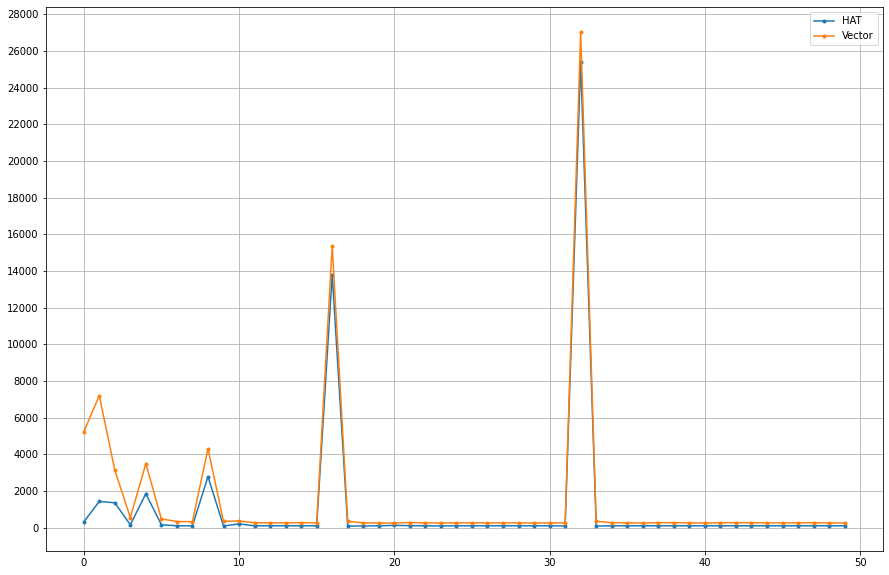
\includegraphics[width=15cm]{p1a}
\end{center}

\part{b} Access Latency \\
HAT $\approx 96$ cycles \\
Vector $\approx 232$ cycles
\begin{center}
  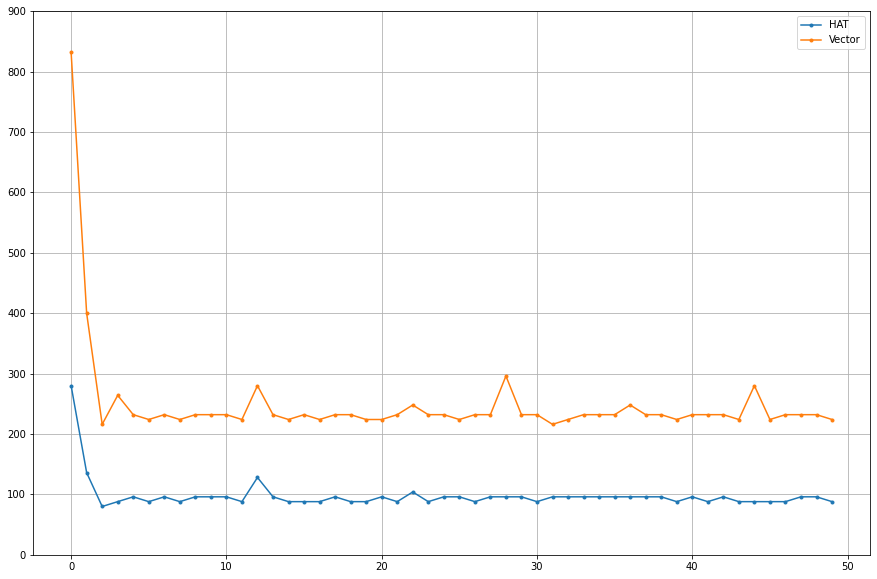
\includegraphics[width=15cm]{p1b}
\end{center}

\part{c} Scan Latency \\
HAT $\approx 1864$ cycles \\
Vector $\approx 2036$ cycles
\begin{center}
  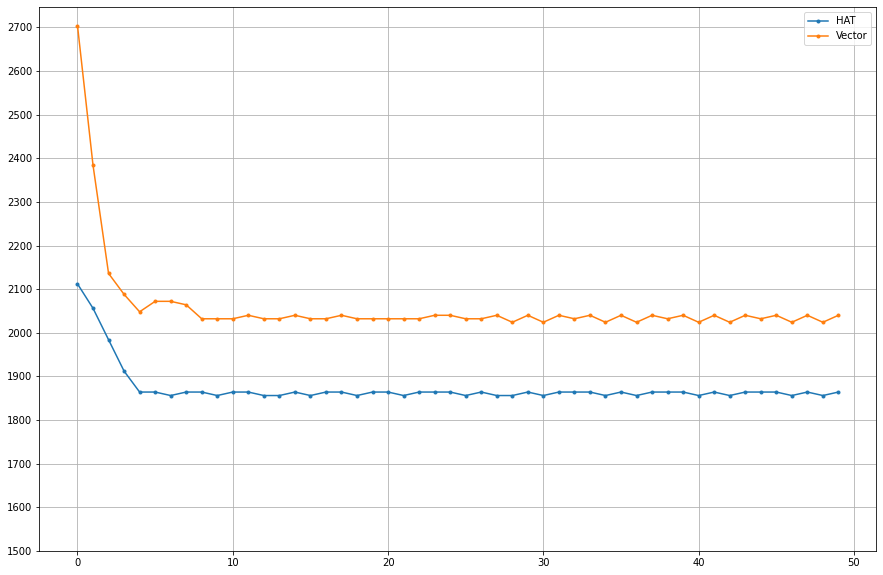
\includegraphics[width=15cm]{p1c}
\end{center}

\part{d}
Overall Latency \\
HAT $\approx 1980$ cycles \\
Vector $\approx 8984$ cycles
\begin{center}
  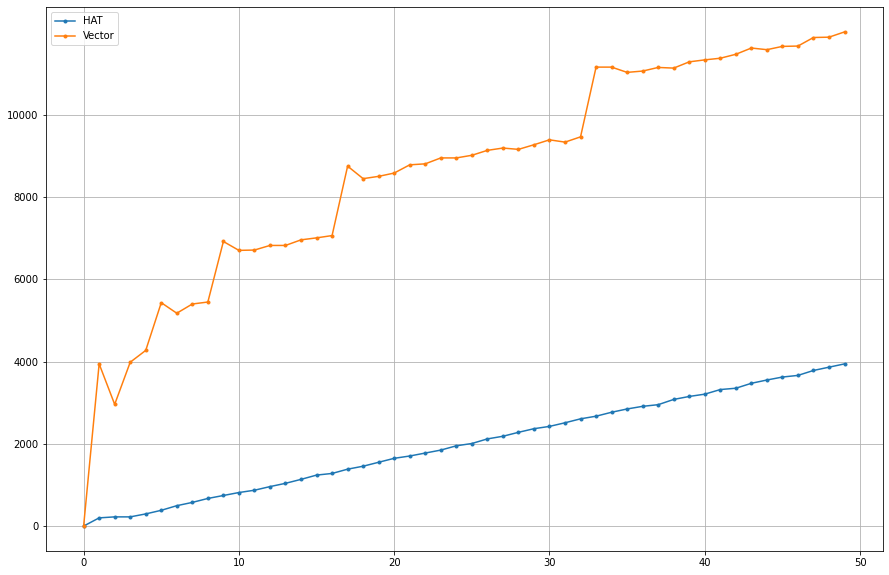
\includegraphics[width=15cm]{p1d}
\end{center}

\question{3}{\textit{Skip Lists}}
\part{a} \\
Insert Latency \\
Skip List $\approx 2236$ cycles \\
Linked List $\approx 2960$ cycles
\begin{center}
  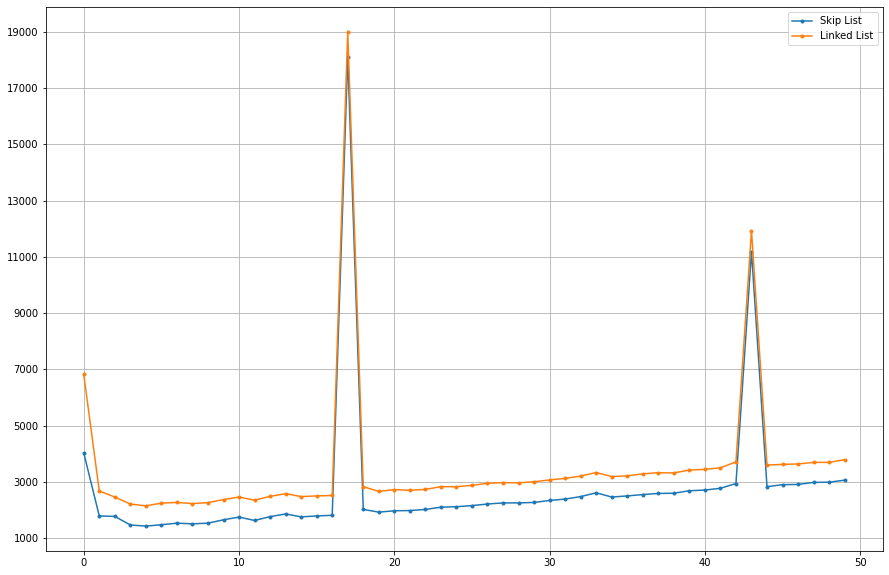
\includegraphics[width=15cm]{p3a1}
\end{center}

Search Latency \\
Skip List $\approx 12212$ cycles \\
Linked List $\approx 65856$ cycles
\begin{center}
  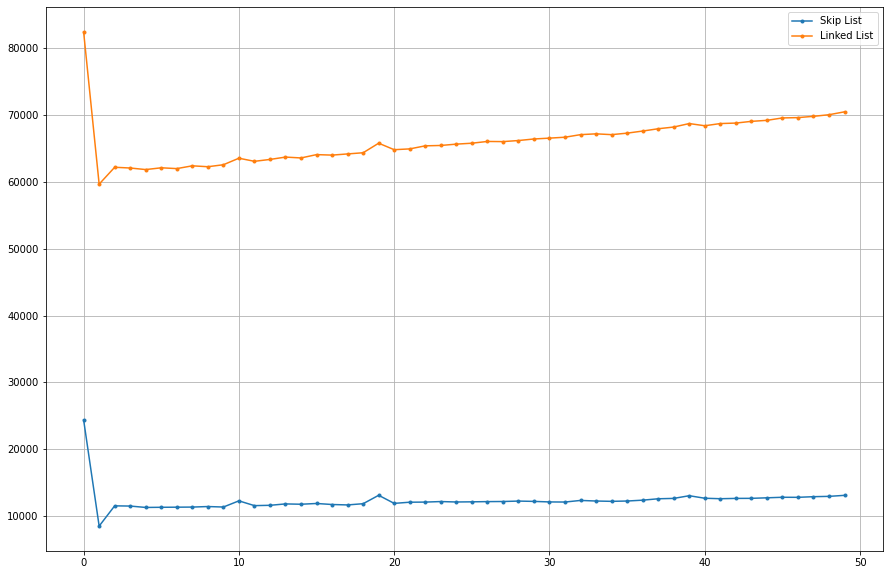
\includegraphics[width=15cm]{p3a2}
\end{center}

\part{b}
Insert Latency $\approx 2556$ cycles \\
\begin{center}
  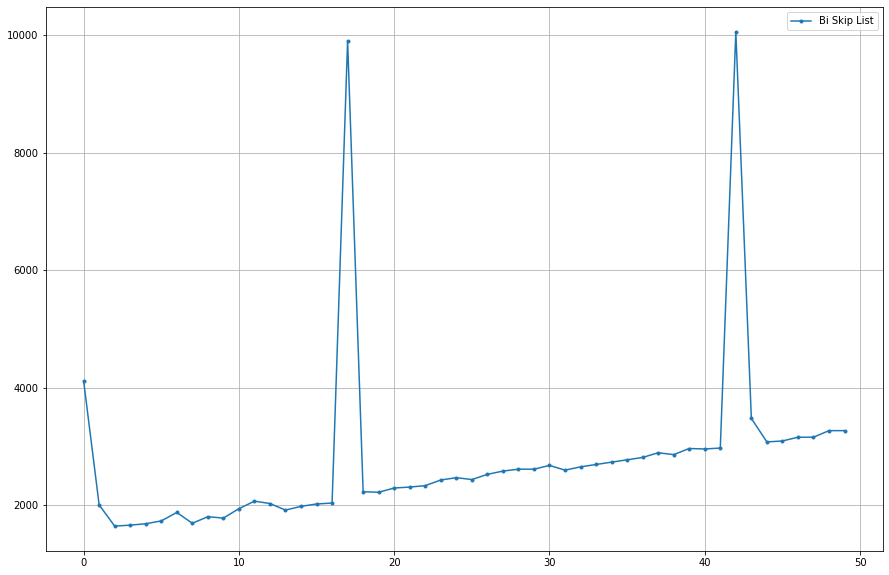
\includegraphics[width=15cm]{p3b1}
\end{center}

Search Latency $\approx 1196$ cycles
\begin{center}
  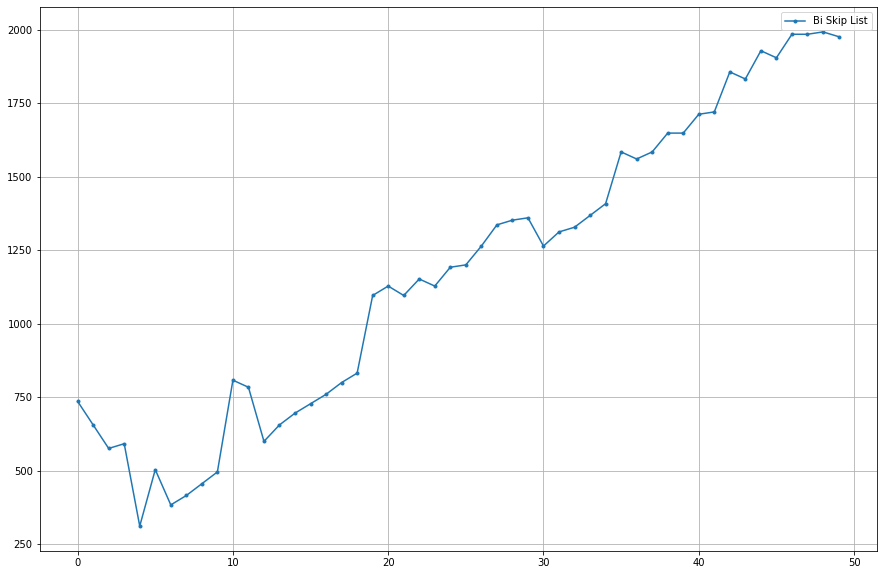
\includegraphics[width=15cm]{p3b2}
\end{center}

\question{4}{\textit{(a, b) tree}}
\part{a} \\
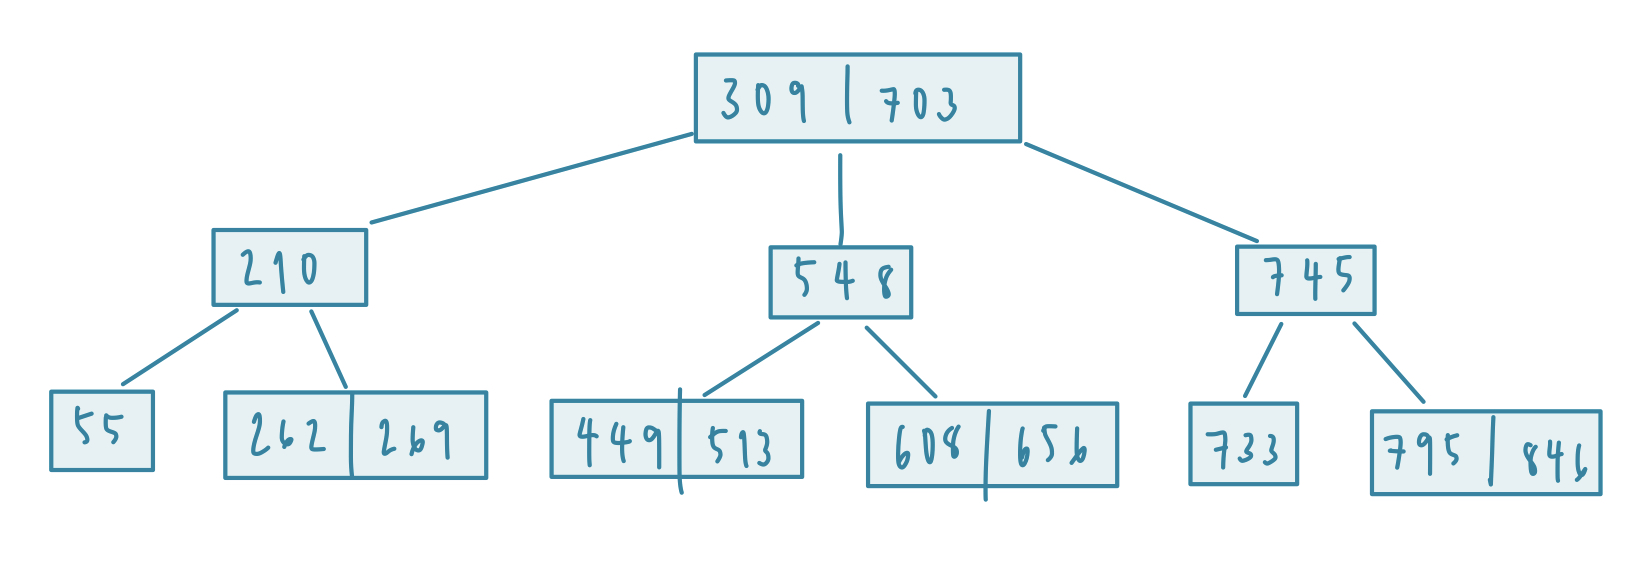
\includegraphics[width=15cm]{p4a}

\part{b} \\
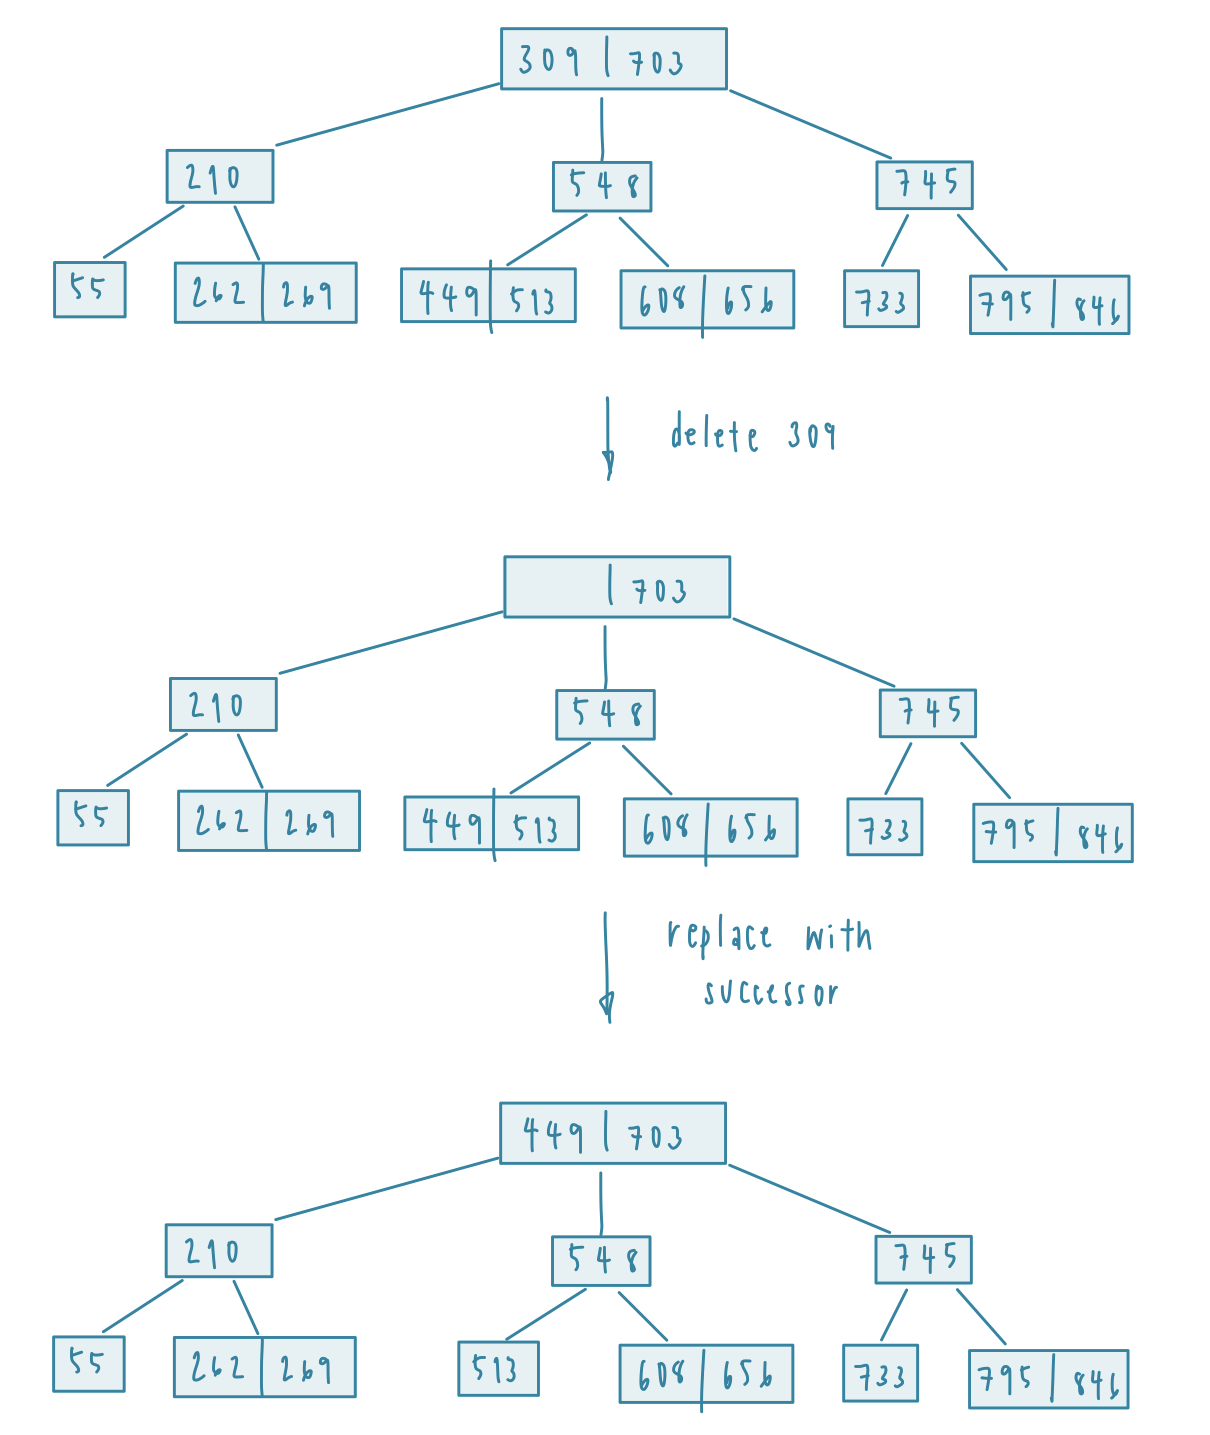
\includegraphics[width=15cm]{p4b}

\question{4}{\textit{B-Tree Speed}}
An optimal value of b should be between 100 and 1000. This range seems to be the balance between minimizing the number of disk accesses and minimizing the space overhead per node.
A smaller value of b means that each node contains fewer keys and values, reducing the space overhead per node. But this also increases the height of the tree, leading to more disk accesses and slower performance for operations that require disk access.
A larger value of b means that each node contains more keys and values, reducing the height of the tree and the number of disk accesses required. However, this also increases the space overhead per node.

\end{document}

